\documentclass[border=10pt]{standalone}
\usepackage{pgfplots}
\pgfplotsset{compat=1.18}
\begin{document}
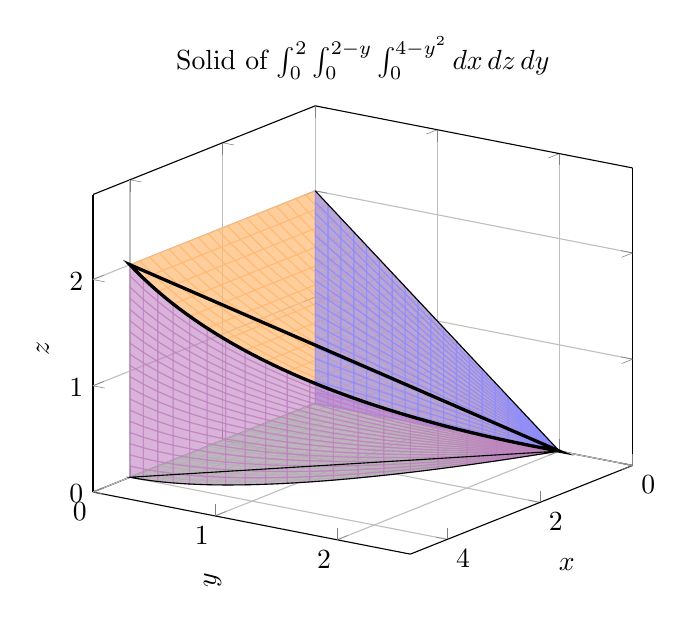
\begin{tikzpicture}
\begin{axis}[
    view={125}{20},
    axis lines = box,
    xlabel = {$x$}, ylabel = {$y$}, zlabel = {$z$},
    xmin=0, xmax=4.8, ymin=0, ymax=2.6, zmin=0, zmax=2.8,
    grid=major,
    title={Solid of $\int_0^2\int_0^{2-y}\int_0^{4-y^2} dx\,dz\,dy$},
]
% Top slanted face z = 2-y, over 0<=x<=4-y^2 (parametric)
\addplot3[surf, shader=flat, faceted color=orange!90, color=orange!55, opacity=0.7,
    domain=0:2, y domain=0:1, samples=20]
    ({(4-x^2)*y}, {x}, {2-x});
% Bottom face z = 0 (green)
\addplot3[surf, shader=flat, faceted color=green!60!black, color=green!40, opacity=0.5,
    domain=0:2, y domain=0:1, samples=20]
    ({(4-x^2)*y}, {x}, {0});
% Back face x = 0 (blue triangle)
\addplot3[surf, shader=flat, faceted color=blue!70, color=blue!45, opacity=0.6,
    domain=0:2, y domain=0:1, samples=20]
    ({0}, {x}, {y*(2-x)});
% Parabolic cylinder face x = 4-y^2 (purple)
\addplot3[surf, shader=flat, faceted color=violet, color=violet!50, opacity=0.6,
    domain=0:2, y domain=0:1, samples=20]
    ({4-x^2}, {x}, {y*(2-x)});
% Intersection curve of z=2-y and x=4-y^2
\addplot3[black, very thick, domain=0:2, samples=40]
    ({4-x^2}, {x}, {2-x});
\addplot3[black, dashed, domain=0:2, samples=40]
    ({4-x^2}, {x}, {0});
\addplot3[black, dashed, domain=0:2, samples=40]
    ({0}, {x}, {2-x});
\end{axis}
\end{tikzpicture}
\end{document}